\section{Literature Review}

\lipsum[2]

\subsection{Non-Intrusive Load Monitoring}

Non-Intrusive Load Monitoring (NILM) also known as energy disaggregation, is a computational techniques that estimates the energy consumed by every individual appliance given just a whole-house power measurements acquired from a single point source such as smart meter. This technique is gaining popularity due to large-scale smart meter deployments worldwide \citep{ReyesLua2015}. 

The big challenge to NILM problem is how to design  algorithm that can accurately perform energy disaggregation. Specifically, the problem of energy disaggregation can be formulated as follows: Given the sequence of aggregate power consumption $\bm{X} = \{X_1,X_2...,X_T \}$ from $N$ active appliances at the entry point of the meter at $\bm{t}=\{1, 2..., T\}$. The task of the NILM algorithm is to infer the power contribution of each of the $N$ appliances, that is,
\begin{gather*}
Y^{(1)} = \{y_1^1, ...,y_T^1\}\\
Y^{(2)} = \{y_1^2, ...,y_T^2\}\\
\vdots \\
Y^{(N)} = \{y_1^N, ..., y_T^N\}
\end{gather*} as shown in Figure \ref{fig:NILM}, such that at any point in time $t$, $$X_t = \sum_{i=1}^N y_t^i + \sigma(t)$$, where $y_t^i$ is the power load of appliance $i$ at time $t$ and $\sigma(t)$ represents both any contribution from appliances not accounted for and measurement noise.
\begin{figure}[ht]
	\centering
	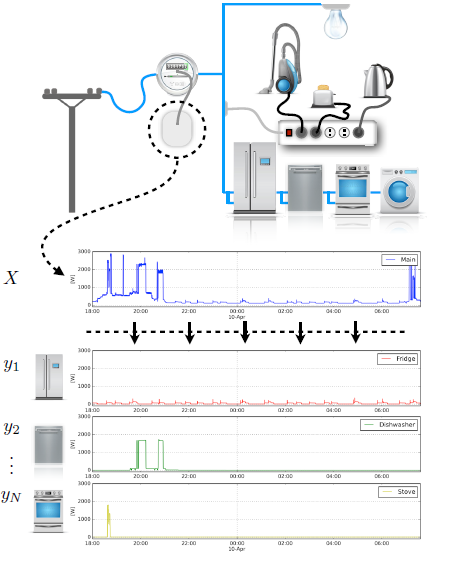
\includegraphics[width=0.5\textwidth]{images/NILM.pdf}
	\caption[An illustration of Non Intrusive Load Monitoring (NILM)]{An illustration of Non Intrusive Load Monitoring (NILM).The goal is to retrieve the individual
		appliance signals $(yi)$ from the total power consumption $X_t$ \citep{Huss2015}}
	\label{fig:NILM}
\end{figure}

A typical NILM algorithm consists of the following steps: power signal acquisition, event detection, feature extraction and inference and learning.

\subsubsection{Power Signal Acquisition}

\lipsum[2]

High-frequency sampling is the measurement of electrical characteristics sampled at a much higher frequency in a range of \SIrange{10}{100}{\mega\hertz}. Power meters at this sampling rates are often custom-built and expensive due to sophisticated hardware \citep{Zoha2012}.

On the other hand, low-frequency sampling is the measurements of the power signal at a rate less than \SI{1}{\hertz}. Smart meters belong to this category since it communicate readings every \SIrange{1}{5}{\second} (\SIrange{0.2}{1}{\hertz}). This research specifically, focus on low-frequency sampling since power data at this sampling can be obtained from smart meters which are being deployed in increasing numbers by utilities worldwide.

\subsubsection{Event Detection}
\lipsum[1]

\textbf{Event-Based Approaches:} The event-based approaches focus on the ON/OFF edges generated by appliances and use change detection algorithm to identify start and end of an event \citep{Barsim2014,Wong2013}.

\lipsum[1]
\begin{figure}[ht]
	\centering
	\includegraphics[width=0.5\textwidth]{images/edge.pdf}
	\caption[Edge-based schematic ]{Schematic of Edge-based \citep{ZhaoyiKang2015}}
	\label{fig:edge}
\end{figure}

\textbf{State-based Approaches:} State-based  State-based NILMs are usually based in HMM and its variants \citep{Kim2011,Kolter2012,Parson2012,Makonin2015} .
\lipsum[2]


\subsection{State-of-the-arts NILM Algorithms}


Several state-of-the-art NILM unsupervised algorithms have been proposed using different approaches such as different variants of Hidden Markov Models (HMM), Graph Signal Processing (GSP) and Deep Neural Networks (DNN). 

\subsubsection{Hidden Markov Model}
HMM is a Markov model whose states are not directly observed instead each state is characterised by a probability distribution function modelling the observation corresponding to that state \citep{Kim2011,Rabiner1989a}. There are two variables in HMM: observed variables and hidden variables where the sequences of hidden variables forms a Markov process. In the context of NILM, the hidden variables are used to model states(ON,OFF, standby etc) of individual appliances and the observed variables are used to model the electric usage. HMMs has been widely used in most of the recently proposed NILM approach because it represents well the individual appliance internal states which are not directly observed in the targeted energy consumption.

A typical HMM is characterised by the following: The finite set of hidden states $S$ (e.g ON, stand-by, OFF, etc.) of an appliance, $S = \{S_1, S_2....,S_N\}$. The finite set of observable symbol $Y$ per states (power consumption) observed in each state, $Y = \{Y_1, Y_2....,Y_M\}$. The observable symbol $Y$ can be discrete or a continuous set. The transition matrix \textbf{A} $=\{a_{ij},1\leq i,j \geq N\} $ represents the probability of moving from state $S_i$ to $S_j$ such that:
$a_{ij} = P(q_{t+1} =S_j \mid q_t=S_i)$, with $a_{ij} \leq 0$ and where $q_t$ denotes the state occupied by the system at time $t$. The emission matrix \textbf{B}$ =\{b(O \mid S_j)\} $ representing the probability of emission of symbol $O$ $\epsilon$ $ Y$ when system state is $S_j$. And the initial state probability distribution $\bm{\pi} = \{\pi_i \}$ indicating the probability of each state of the hidden variable  at $t = 1$ such that, $\pi _i = P(q_1 = s_i), 1 \leq i \geq N$. 

The set of all HMM model parameters is represented by 
$\bm{\lambda =\{\pi, A, B \}}$.~Several HMMs based NILM algorithms for energy disaggregation at low sampling rate has been proposed in the literature.


\cite{Kim2011} propose  an unsupervised technique for energy disaggregation using a combination of four FHMM variants. They use low-frequency real power feature and assume a binary state of appliances. To learn model parameters, Kim's approach uses Expectation Maximasation(EM) algorithm  and employ Maximum Likelihood Estimation(MLE) algorithm to infer load states. The performance of Kim's technique quickly decreases as the number of appliances increases and can only identify up to 10 appliances \citep{Parson2014c}. In addition, the reported work require appliances to be manually labelled after disaggregation and suffer from high computational complexity which makes it unstable for real-time applications.



\subsection{Energy Datasets}
\lipsum[1] 

Recent years has seen the emergency of several publicly available datasets such as UK-DALE \citep{Kelly2015}, AMPDs and AMPDs2 \citep{Makonin2013,Makonin2016}, ECO dataset \citep{Beckel2014}, REFIT dataset \citep{Murray2015b} and GREED dataset \citep{Monacchi2015a}. The comparison of various publicly available dataset with their characteristics is shown in Table \ref{tab:dataset}. This comparison is an extension of the proposed one in \citep{Bonfigli2015} and \citep{Murray2015b} with an update of the recent published data and additional data on included in some datasets. However, most of the datasets are from USA and some from European countries besides Canada and India. To the knowledge of researcher, there is no open-access dataset recorded in Tanzania. According to \cite{Kelly2015} to test the performance of a NILM algorithm for a specific country, it is important to have access to data from that country. This is because electricity usage varies significantly between countries owing to different use of sets of appliances and different cultures. Using dataset recorded from different countries could lead to mismatching of electric quantities. For example, while most of existing datasets recorded from USA where the RMS voltage value is \SI{120}{\volt}, most of developing countries including Tanzania work under \SI{240}{\volt} RMS voltage. The study will develop energy data set containing detailed power usage information obtained from well-instrumented residential buildings in Tanzania. Availability of these data set will promote research activities in energy consumption, data analysis and provide understanding of Tanzania domestic power usage and consumption.

\begin{landscape}
	\begin{table}[]
		\centering
		\caption{Publically Available Energy Dataset Comparison}
		\scalebox{0.75}{
			\begin{tabular}{p{4cm}p{2cm}p{3cm}p{2cm}p{3cm}p{5cm}p{5cm}p{7cm}}
				\toprule
				Dataset & Location & Duration & Number of houses & Sensors per house & Sample resolution & Features & Other Data \\
				\midrule
				REDD \citep{Kolter2011} & USA & 3-19 days & 6 & 24 & 15KHz(Aggr), 0.5Hz and 1Hz (sub) & V and P (Aggr), P (sub) &  \\
				BERDS \citep{Maasoumy2013} & USA & 1 year & 1 & 4 & 20sec & P,Q and S & climate data \\
				BLUED \citep{Anderson2012a} & USA & 8 days & 1 & Aggregated & 12KHz(Aggr only) & I, V and State transition label for each appliance. &  \\
				Smart \citep{Barker2012a} & USA & 3 months & 3 & 21-26 circuit meters & 1Hz & P and S (Aggr), P (Sub) & electricity generation data from on-site solar panels and wind turbines, outdoor weather data, temperature and humidity data in indoor rooms \\
				Tracebase \citep{Reinhardt2012} & Germany & N/A & 15 & 158 devices & 1-10sec(Sub only) & P &  \\
				AMPDS \citep{Makonin2013} & Canada & 1 year & 1 & 19 & 1min & V, I, F P, Q, S and Pf & water and natural gas, \\
				AMPds2 \citep{Makonin2016} & Canada & 2 & 1 & 21 & 1min & V, I, F P, Q, S , Pf ,real energy, reactive energy, and apparent energy & water and natural gas, weather data and   utility billing data. \\
				UK-DALE \citep{Kelly2015} & UK & 499 days, 2.5 years(house 1) & 5 & 5-54 devices & 16 kHz(Aggr) and 1/6 Hz(Sub) & P and switch status &  \\
				iAWE \citep{Batra2013} & India & 73 days & 10 & 33 devices & 1sec(Aggr) and 1sec or 6sec (Sub) & V, I, F, P and phase & Water and ambient conditions \\
				REFIT \citep{Murray2015} & UK & 2years & 20 & 11 & 8sec & P & Gas and environmental data \\
				GREED \citep{Monacchi2015a} & Australia/Italy & 1year & 9 & 9 & 1Hz & P &  \\
				ECO \citep{Beckel2014} & Switzerland & 8months & 6 &  & 1Hz & P and Q & Occupancy information \\
				IHEPCDS \footnote{http://archive.ics.uci.edu/ml/datasets/Individual+household+electric+power+consumption} & France & 4 years & 1 & 3 & 1min & V, I, P and Q &  \\
				OCTES \footnote{http://octes.oamk.fi/final/} & Scotland,Iceland \&Finland & 4–13months & 33 & Aggregated & 7sec & P and phase &  \\
				HES & UK & 1month(255 houses), 1year(26houses) & 251 & 13-51 & 2min & P &  \\
				ACS-F1 \citep{Gisler2013} & Switzerland & 2, 1 hoursessions & NA & 100, 10 types & 10sec & P, Q, I, f, V and phase & \\
				\bottomrule 
			\end{tabular}%
		}
		\label{tab:dataset}%
		\raggedright{\textit{Aggregte (Aggr), Sub-metering (sub), Active Power (P), Reactive Power (Q), Apparent Power (S), Energy (E), Frequency (f), Voltage (V) and Current (I)}}
	\end{table}
\end{landscape}
\subsection{Conclusion}
Despite the major leaps forward in the field, the electricity disaggregation problem is by no means solved; no convincing results have been presented for a precise and reliable method that is general enough to be deploy in any household.






















































































































































































































































































































































































































































































































































































































































































































